\documentclass{hw}
\usepackage{amssymb,listings,xcolor,graphicx}
\title{Homework 2}
\course{ECEN 2020}
\author{Patrick Harrington}
\renewcommand\thesubsection{(\alph{subsection})}
\lstset{ 
  language=C,
  basicstyle=\fontfamily{pcr}\selectfont\footnotesize\color{black},
  keywordstyle=\color{black}\bfseries, % style for keywords
  numberstyle=\tiny\color{gray},
  rulecolor=\color{black},
  numbers=left, numberstyle=\tiny, 
  frame=single,
  tabsize=2
}
\begin{document}
\maketitle
\section{Blink Program}
  Yes; program works on Arduino Uno as intended.
\section{Name Program}
  See attached files.
\section{Modified Blink}
  See attached files.
\section{Transform Step}
\begin{lstlisting}
void setup() {}
void loop() { my_function();}
void my_function()
{
  void setup(){
    Serial.begin(9600);
  }

  void loop(){
    Serial.println(``AM I BEING ANNOYING?'');
    delay(1000);
  }
}
\end{lstlisting}

After running \texttt{ino build}, the following \texttt{.cpp} file was output
after a transformation in the build process:

\begin{lstlisting}
#include <Arduino.h>
void setup();
void loop();
#line 1 ``src/sketch.ino''
void setup(){
  Serial.begin(9600);
}
  
void loop(){
  Serial.println(``AM I BEING ANNOYING?'');
  delay(1000);
}
\end{lstlisting}
\section{Serial.begin(9600)}

9600 represents the \textbf{Baud rate} (in units of symbols per second). The
number 9600 is one of historical relevance and is used today for compatability
reasons. The function itself is used to establish serial communications with a
computer, the argument being the rate.

\section{Secondary Serial Monitor}

Since I have been using \texttt{ino} for most of my work on the Arduino, I have
been using \texttt{picocom} to talk to the Arduino. In Figure~\ref{shot}, a
screenshot of picocom in action is shown.

\begin{figure}[ht!]
  \centering
  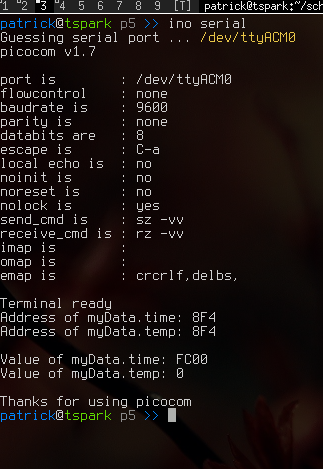
\includegraphics[scale=0.7]{shot.png}
  \caption{A screenshot of \texttt{picocom} in use}
  \label{shot}
\end{figure}

\end{document}

